% !TeX root = ../dokumentation.tex

\chapter{Sprints}

\section{Sprint 1}
\todo{Beschreibung des Produktincrements}

\section{Ziele Sprint 1}
\todo{Ziel Sprint 1}

\section{Ergebnisse Sprint 1}

\subsection{Produktincrement}
\subsection{Charts}

\subsection{Probleme und Verbesserungen}
\todo{Retro Ergebnisse}


\subsection{Bearbeitete User Storys}

\subsubsection{Ticket 1}

\subsubsection{Ticket 2}

\subsubsection{SKIOS-13 Create Basic Infrastructure}
Das Ticket \enquote{SKIOS-13 Create Basic Infrastructure} hatte folgende User Story:
\begin{quotation}
    Create Basic Server Infrastructure:
    Domain Setup
    Server Setup (SSH Config & Firewall)
    Install Basics Tools
    Install k3s without any settings
    Setup remote access to k3s
\end{quotation}
Dies wurde folgendermaßen gelöst:
\begin{quotation}
    
\end{quotation}
Bearbeitet von Lukas Huida.

\subsubsection{SKIOS-18 Basic Kubernetes Infra}
Das Ticket \enquote{SKIOS-18 Basic Kubernetes Infra} hatte folgende User Story:
\begin{quotation}
    As a infra member I want a basic Infrastructure based on Kubernetes.
    Acceptance Criteria
    Working Ingress-Controller with correct Certs
    Repo with examples
    Own Docker-Registry
    Setup ArgoCD
    Setup Drone.io
    Setup SonarQube
    Setup HashiCorp Vault (Optional)
    Setup keycloak (Optional)
\end{quotation}
Dies wurde folgendermaßen gelöst:
\begin{quotation}
    
\end{quotation}
Bearbeitet von Lukas Huida.

\subsubsection{SKIOS-9 Create Continous Integration Pipeline}
Das Ticket \enquote{SKIOS-9 Create Continous Integration Pipeline} hatte folgende User Story:
\begin{quotation}
    As a developer I want my code to be tested and analyzed by sonar after every new commit so that our platform can ensure stability.
    Acceptance Criteria
    code of branches in pull requests trigger a pipeline after every commit
    the pipeline runs through: (1) unit tests (2) integration tests (3) sonar qube
    build container
    To be clarified
    When should we trigger this pipeline? After every commit, before merging, etc.?
    Can we actually do integration tests or is this out of scope?
    Notes
    Unit Tests
    Docker Image
    Integration Test (postman → newman runner)
    Mock Database?
    Mock Keycloak?
    Code Coverage (ex. SonarQube → has code-smell function)
    Trigger Pipeline → pr & commit on branches != master (optional)
    Optional Trigger CD Script/Pipeline to roll-out new docker-image after commit to master
\end{quotation}
Dies wurde folgendermaßen gelöst:
\begin{quotation}
    
\end{quotation}
Bearbeitet von Lukas Huida.

\subsubsection{SKIOS-10 Create Continous Delivery Pipeline}
Das Ticket \enquote{SKIOS-10 Create Continous Delivery Pipeline} hatte folgende User Story:
\begin{quotation}
    As a developer I want my code to be delivered to prod after I merge it to master.
    Acceptance Criteria
    pipeline is triggered after merge to master
    pipeline tests code with unit/sonar before merge (is already managed by ci-pipeline)
    pipeline tests code with newman after merge -> fail leads to rollback
    To be clarified
    Should we actually deploy to prod every time - yesAre rollbacks out of scope for the initial infrastructure - will be handled in a separate story later on
\end{quotation}
Dies wurde folgendermaßen gelöst:
\begin{quotation}
    
\end{quotation}
Bearbeitet von .

\subsubsection{SKIOS-21 Initialize Keycloak}
Das Ticket \enquote{SKIOS-21 Initialize Keycloak} hatte folgende User Story:
\begin{quotation}
    As a developer I would like to have keycloak setup so that we can test its usefullness.
    Acceptance Criteria
    Keycloak server is running in our cluster
    Keycloak intercepts all backend calls (through nginx gateway etc)
    Open Questions
    Should we add making some type of test request to the Acceptance criteria or not?
\end{quotation}
Dies wurde folgendermaßen gelöst:
\begin{quotation}
    
\end{quotation}
Bearbeitet von Lukas Huida.

\subsubsection{SKIOS-30 Preliminary Core service}
Das Ticket \enquote{SKIOS-30 Preliminary Core service} hatte folgende User Story:
\begin{quotation}
    Create a boilerplate for core service with mock endpoints for what is needed in frontend
    be able to fetch article with graphql
\end{quotation}
Dies wurde folgendermaßen gelöst:
\begin{quotation}
    
\end{quotation}
Bearbeitet von Lukas Huida.

\subsubsection{SKIOS-37 Decision of Programming Database}
Das Ticket \enquote{SKIOS-37 Decision of Programming Database} hatte folgende User Story:
\begin{quotation}
    As a developer I need to know which Database is used, to know which database connector for ORMs are needed
    Acceptance Criteria
    A decision of a Database is done
    The decision is documented in Confluence
\end{quotation}
Dies wurde folgendermaßen gelöst:
\begin{quotation}
    
\end{quotation}
Bearbeitet von Lukas Huida.

\subsubsection{SKIOS-49 Create Example Service}
Das Ticket \enquote{SKIOS-49 Create Example Service} hatte folgende User Story:
\begin{quotation}
    Code example service
    Create Deployment for example service
    Create Repo with CI Pipeline
    Docker Credentials
\end{quotation}
Dies wurde folgendermaßen gelöst:
\begin{quotation}
    
\end{quotation}
Bearbeitet von Lukas Huida.

\subsubsection{SKIOS-50 Deploy Database}
Das Ticket \enquote{SKIOS-50 Deploy Database} hatte folgende User Story:
\begin{quotation}
    As a developer I want a central Database to store my Objects and Articles.
    Acceptance Criteria
    postgresql is deployed in a db namespace
    db is reachable in the default namespace with credentials stored at the vault
\end{quotation}
Dies wurde folgendermaßen gelöst:
\begin{quotation}
    
\end{quotation}
Bearbeitet von Lukas Huida.

\section{Sprint 2}
\subsection{Produktincrement}
\subsection{Charts}
\subsection{Probleme und Verbesserungen}


\subsection{Bearbeitete User Storys}

\subsubsection{SKIOS-67 Enhanced Git/Jira Automation}
Das Ticket \enquote{SKIOS-67 Enhanced Git/Jira Automation} hatte folgende User Story:
\begin{quotation}
    As a developer I would like enhanced integration for Jira.
    Automation to auto. change the following types:
    Dev starts new Branch for his work, Story changes status to → in progress
    Dev starts PR for his Story → Story changes status to → needs review
    PR is merged → Story changes status to → done
    Sync Reviewer between Jira & Git (optional)
    Acceptance Criteria
    Requirements above are covered
    functionality works for all projects
\end{quotation}
Dies wurde folgendermaßen gelöst:
\begin{quotation}
    
\end{quotation}
Bearbeitet von Lukas Huida.

\subsubsection{SKIOS-69 Preliminary ORM}
Das Ticket \enquote{SKIOS-69 Preliminary ORM} hatte folgende User Story:
\begin{quotation}
    Als Programmierer will ich eine Datendefinition in einer Datenbank
    haben, und diese als Packet einbinden können.
\end{quotation}
Diese wurde folgendermaßen gelöst:
\begin{quotation}
Die Datendefinition wurde durch TypeORM~\parencite{web/TypeORM} dargestellt.
Diese wurde in dem Repository skiosa/orm~\parencite{git/skiosa/orm} als NPM-Package~\parencite{web/npm} abgebildet.
Es wurden die Article von RSS-Feeds in dem Schema aus Abbildung~\ref{fig:databaseORM} abgebildet.
\begin{figure}
    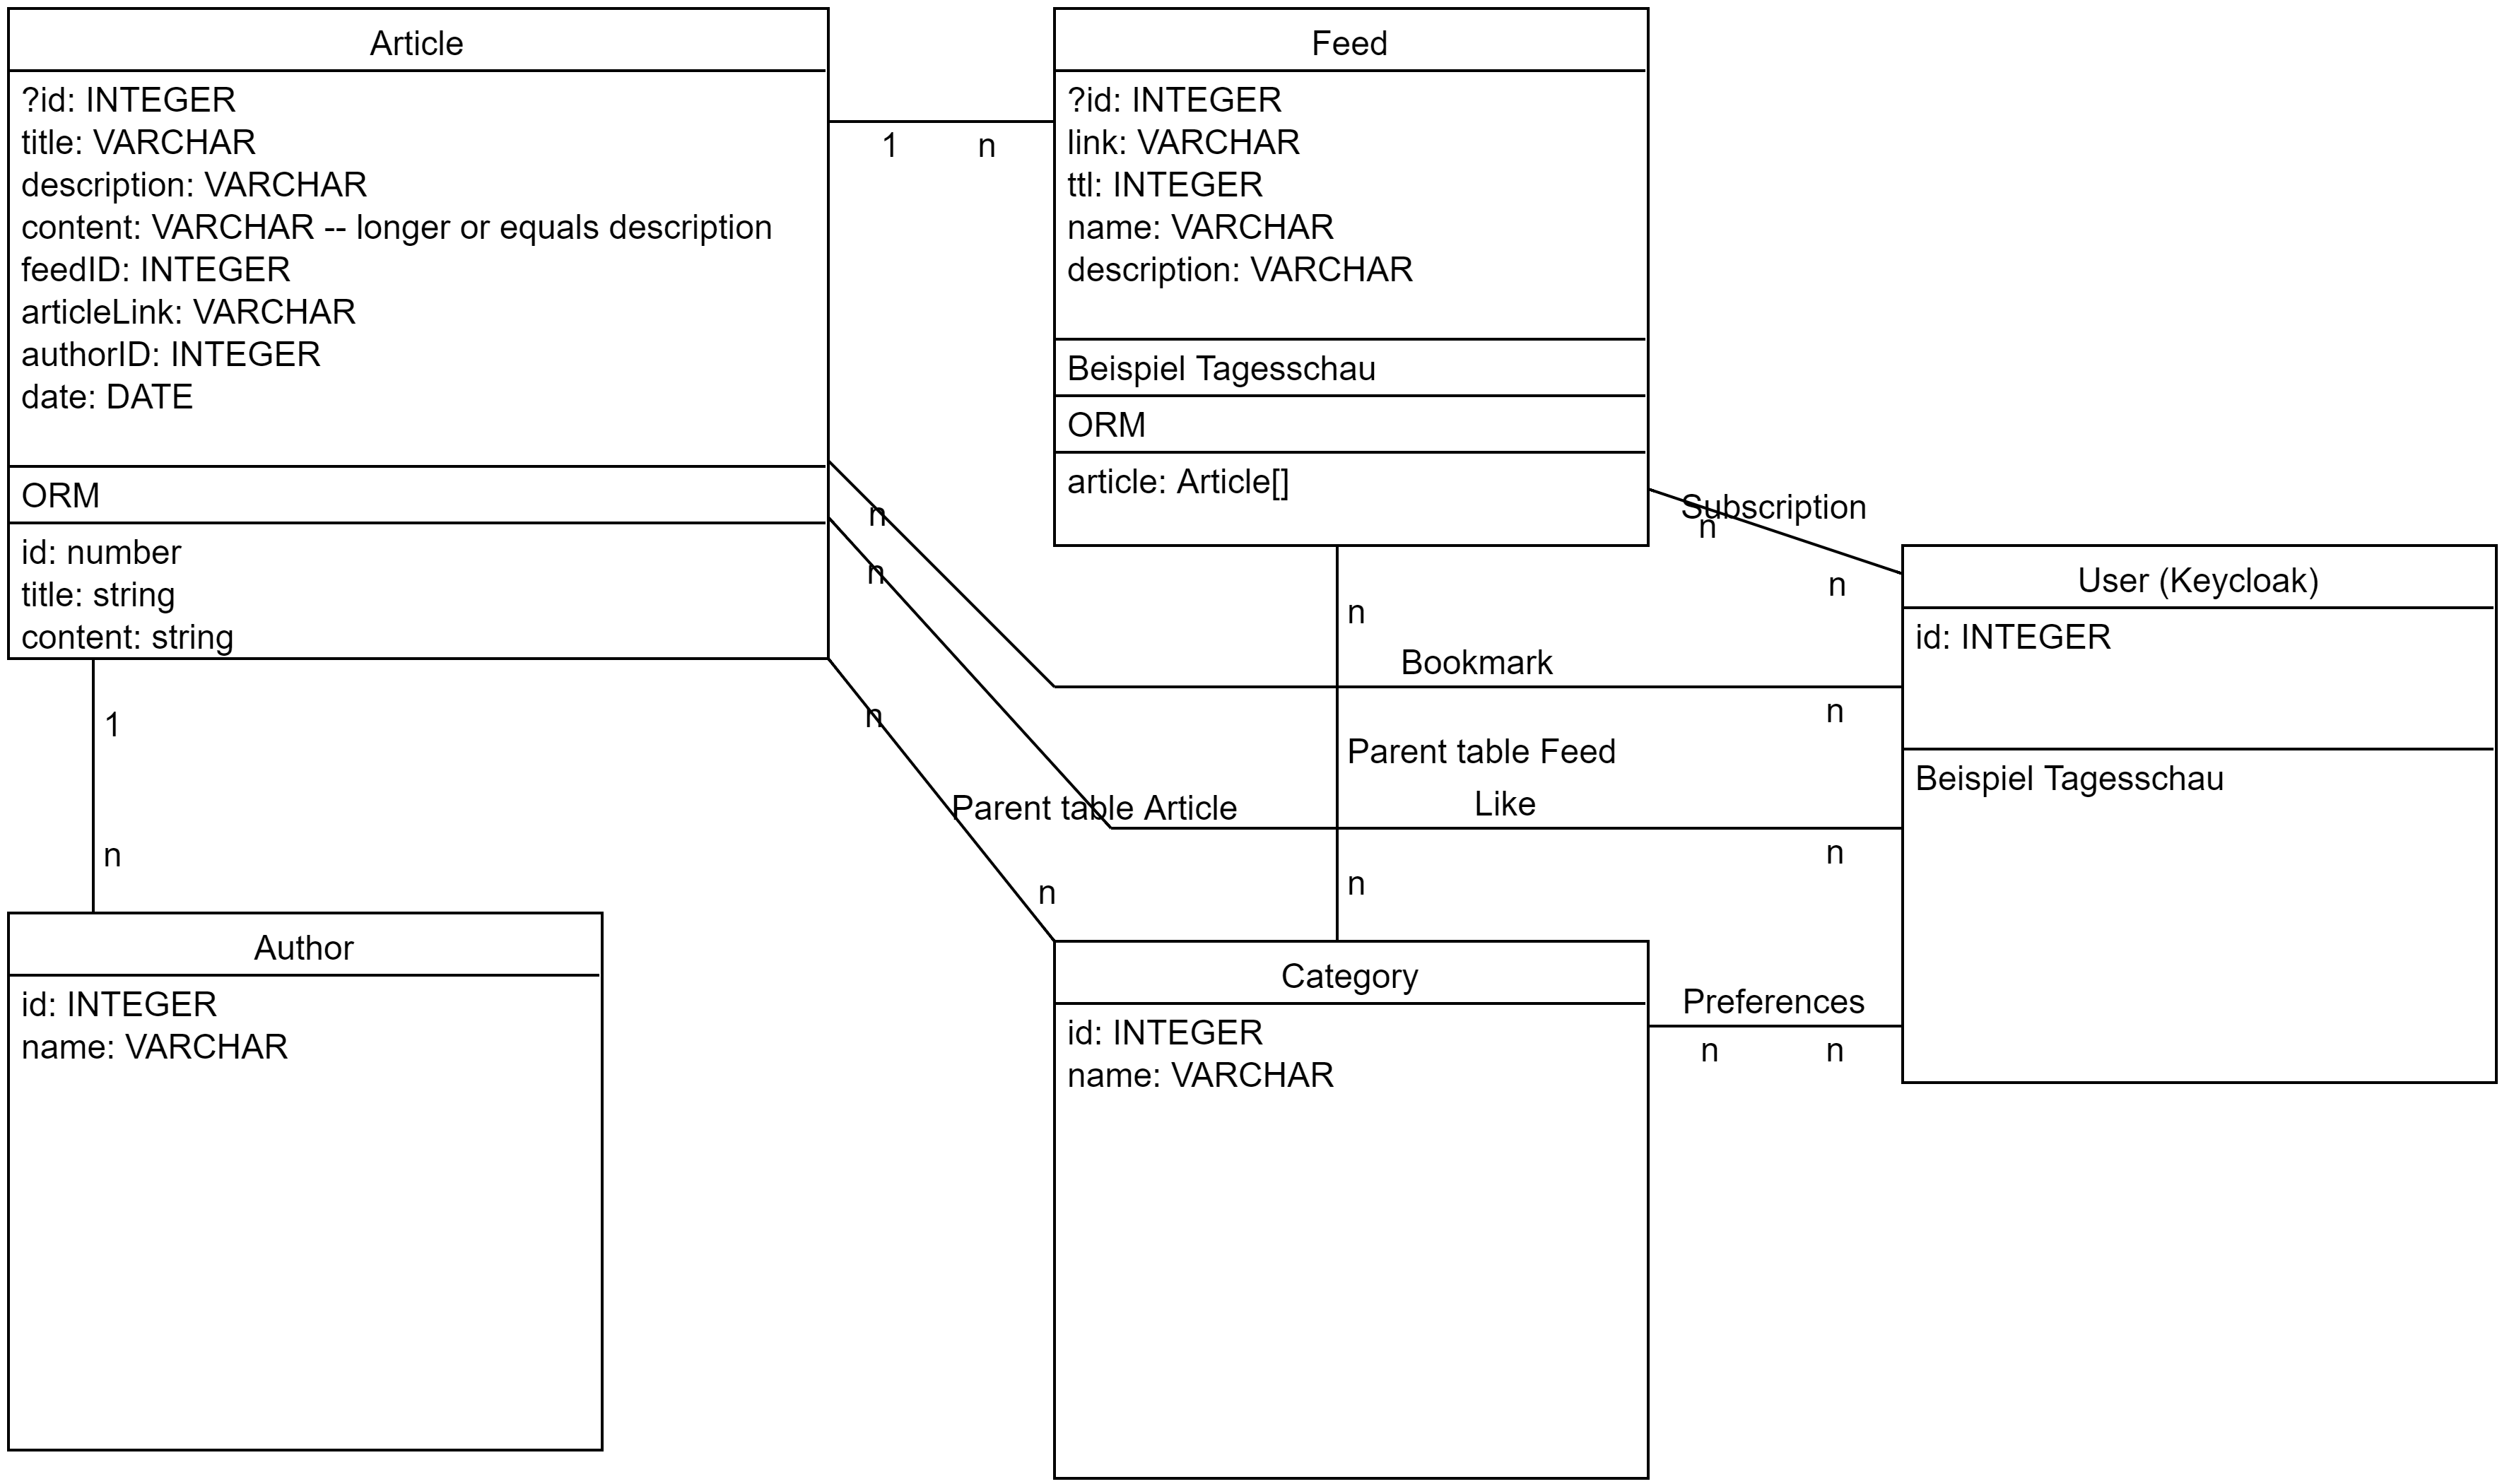
\includegraphics[width=\linewidth]{Database_Model.png}
    \caption{Datendefinition innerhalb der Datenbank}
    \label{fig:databaseORM}
\end{figure}
\end{quotation}
Bearbeitet von Jonas Eppard und Tim Horlacher.

\subsubsection{SKIOS-74 Extend workflow to include wontfix}
Das Ticket \enquote{SKIOS-74 Extend workflow to include wontfix} hatte folgende User Story:
\begin{quotation}
    As a team member, I would like a wontfix state  to disregard tickets.
    Goal of this story is to modify the current issue workflow used by jira
    Note: this might require admin rights (contact PO or Architect for this)
    Acceptance Criteria
    Wontfix status exists
    The status contains the “done” property (is striked out)
\end{quotation}
Dies wurde folgendermaßen gelöst:
\begin{quotation}
    
\end{quotation}
Bearbeitet von Lukas Huida.

\subsubsection{SKIOS-85 Repeated Polling runs}
Das Ticket \enquote{SKIOS-85 Repeated Polling runs} hatte folgende User Story:
\begin{quotation}
    As a developer I would like the polling service to be run as a cron job.
    Acceptance Criteria
    Polling service is called in intervalls
    Pod isnt running all the time
\end{quotation}
Dies wurde folgendermaßen gelöst:
\begin{quotation}
    
\end{quotation}
Bearbeitet von Lukas Huida.

\section{Sprint 3}

\subsection{Produktincrement}
\subsection{Charts}
\subsection{Probleme und Verbesserungen}


\subsection{Bearbeitete User Storys}
\subsubsection{SKIOS-116 Structure and table of contents for submission (\LaTeX)}
Das Ticket \enquote{SKIOS-116 Structure and table of contents for submission (\LaTeX)}
hatte folgende User Story:
\begin{quotation}
    As a team member, I would like to have a rough structure to orient myself while writing our submission documentation.\\
    For this story, please read the requirements and guidelines set out by Garidis and develop a rough idea on how to structure our \LaTeX project.\\
    \textbf{Acceptance Criteria}
    \begin{itemize}
        \item Table of contents is created (with \textbackslash{}section, \textbackslash{}subsection, etc.) in \LaTeX
        \item Structure reflects guidelines of Garidis
        \item Structure is explained in confluence page
        \item Existing \LaTeX~stories have a defined place where their pages will go
    \end{itemize}
\end{quotation}
Dies wurde folgendermaßen gelöst:
\begin{quotation}
    Es wurde die Struktur dieses \LaTeX-Dokuments angelegt. Hierbei musste nur das Inhaltsverzeichnis
    angelegt werden, da das \LaTeX-Template schon vorhanden war.
    Die Verwendung wurde in Confluence dokumentiert.
\end{quotation}
Bearbeitet von Jonas Eppard.

\subsubsection{SKIOS-73 Place new logo in git, jira, confluence, etc}
Das Ticket \enquote{SKIOS-73 Place new logo in git, jira, confluence, etc} hatte folgende User Story:
\begin{quotation}
    Add branding for skiosa
    possibly also change look of Jira (at the top) and make it use our colorscheme
    Acceptance Criteria
    Skiosa Brandig is present in Git and Jira
\end{quotation}
Dies wurde folgendermaßen gelöst:
\begin{quotation}
    
\end{quotation}
Bearbeitet von Lukas Huida.

\subsubsection{SKIOS-76 Automatic Reviewer Suggestions}
Das Ticket \enquote{SKIOS-76 Automatic Reviewer Suggestions} hatte folgende User Story:
\begin{quotation}
    use git automatition to automatically suggest a reviewer based on recent committers to that service or topic
\end{quotation}
Dies wurde folgendermaßen gelöst:
\begin{quotation}
    
\end{quotation}
Bearbeitet von Lukas Huida.

\subsubsection{SKIOS-91 Checklist for PRs}
Das Ticket \enquote{SKIOS-91 Checklist for PRs} hatte folgende User Story:
\begin{quotation}
    As a developer I would like a reminder to check off the checklist from our contributing guidelines.
    Acceptance Criteria
    Every PR contains comment or default text including the checklist
\end{quotation}
Dies wurde folgendermaßen gelöst:
\begin{quotation}
    
\end{quotation}
Bearbeitet von Lukas Huida.

\subsubsection{SKIOS-138 Use Keycloak in GraphQL}
Das Ticket \enquote{SKIOS-138 Use Keycloak in GraphQL} hatte folgende User Story:
\begin{quotation}
    ja.
\end{quotation}
Dies wurde folgendermaßen gelöst:
\begin{quotation}
    
\end{quotation}
Bearbeitet von Lukas Huida.
